\section{Deployment View}
THis part of the \emph{Design Document} is devoted to explain at the best the four tiers that compose the \emph{Travlendar+} system.

First of all, the application is created to work either on a web browser or on a mobile phone through an application.
To have a system which is easily maintainable, both the clients will implement the \emph{REST} protocol, with an \emph{HTTPS} communication, in this way the mobile application and the web server can change their internal component, and the only thing to taking into account is to implement the correct \emph{RESTful} services.

The clients send requests to the \emph{Travlendar+} web server, in which there is the \emph{Server Façade}, a component use to receive messages from the Internet and to send them to the \emph{Application Server}.

The \emph{Application Server} is the server that contains all the \emph{Business Logic} components. This layer runs the main functionalities of the \emph{Travlendar+}, and also is used to access to the internal database, to store useful user's datas. Notice that the \emph{Application Server} is in a \emph{demilitarized} zone (DMZ), in order to avoid some possible hacks from the Internet. In this zone also the \emph{Database Server} takes place, in this way the important datas are stored in a secure way.

Finally the \emph{Application Server} is also used to communicate with the \emph{External Services}. These services are helpful to the core features of \emph{Travlendar+}. Indeed the application needs to know the best travel, with additional information (such as the estimated travel time and the expected traffic); the travel means, with their time tables, and finally the various tickets' costs.

\begin{figure}[H]
    \centering
    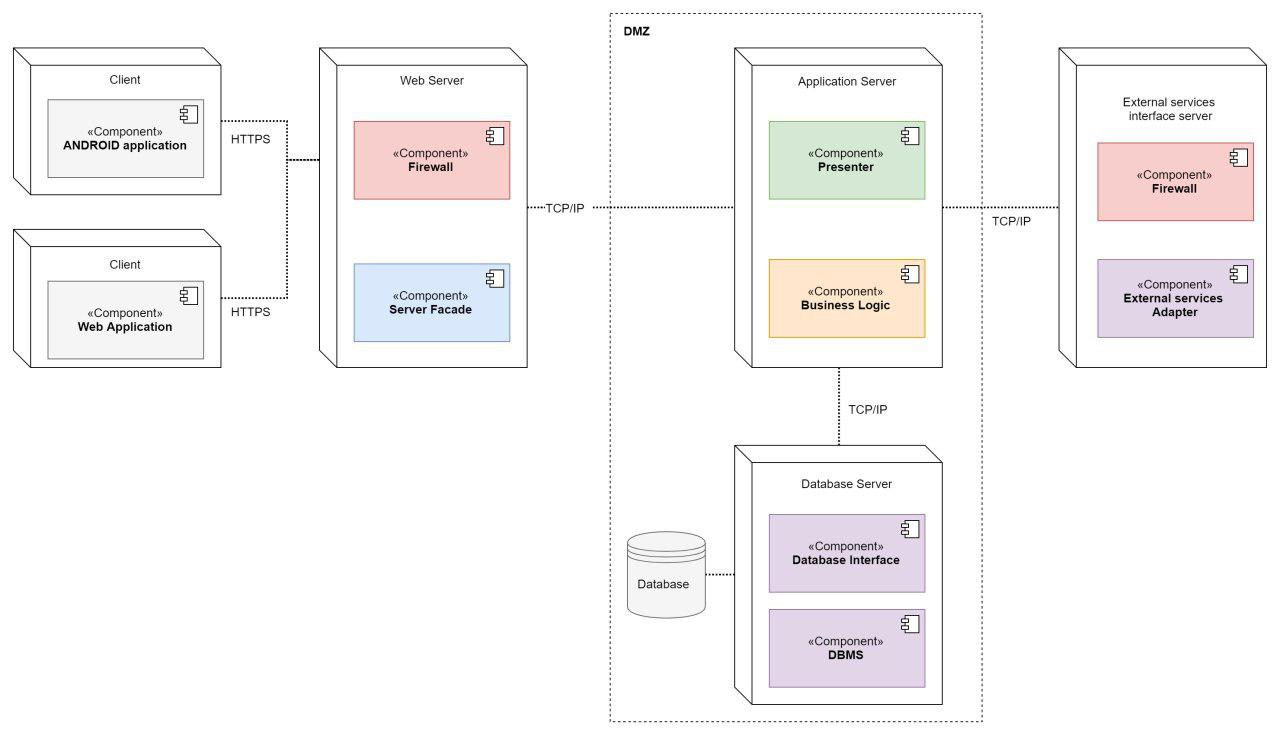
\includegraphics[scale=0.9]{Pictures/DeploymentPictures/deploymentDiagram.jpg}
    \caption{Deployment Diagram for \emph{Travlendar+} System}
\end{figure}